\section{Locus Triple Winding}
\label{sec:05-triple-winding}

Consider one turn of vertex $P_1(t)$ of billiard 3-periodics around the billiard. Given 3-periodic triple periodicity, over said motion a triangle center will sweep its locus thrice (excluding $X_9$ which doesn't move).

Referring to \cref{fig:05-intouch-rho}, consider the convex combination $Y_1(t)$ of incenter $X_1$ and an intouch point $I_1(t)$, namely:

\[ Y_1(t) = (1-\rho) X_1(t) +  \rho I_1(t)  \]
where $\rho$ is a real number.

\begin{figure}
    \centering
    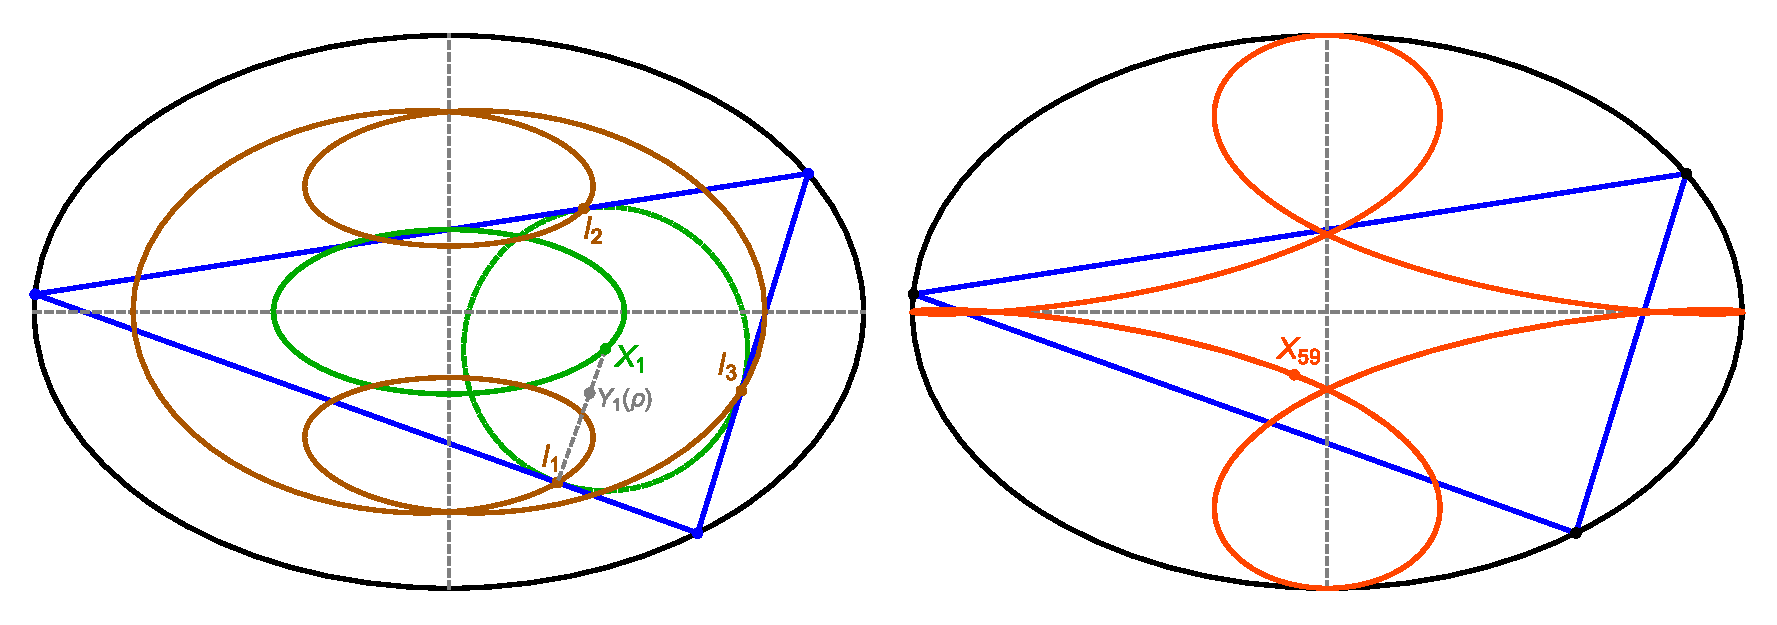
\includegraphics[trim=0 0 425 0,clip,width=.6\textwidth]{pics_05_010_x1_x59.eps}
    \caption{Depicted is the convex combination $Y_1(\rho)$ of the incenter $X_1$ and an intouchpoint $I_1$ of a billiard 3-periodic.  \href{https://bit.ly/3q4b0Nn}{app},  \href{https://youtu.be/BBsyM7RnswA}{Video 1}, \href{https://youtu.be/9xU6T7hQMzs}{Video 2}.}
    \label{fig:05-intouch-rho}
\end{figure}

Loci obtained for $Y_1$ at different values of $\rho$ are shown in \cref{fig:05-inc-wind3}. At $\rho=1$ (top-left), $Y_1(t)$ is the recognizable two-lobe locus of the intouchpoints. As $\rho$ decreases, the two lobes approach each other. At some critical $\rho$ they will touch each other at single point. Decreasing $\rho$ further causes the lobes to self-intersect and contain the center of the confocal ellipse pair,. which entails that the turning number about the origin of the locus suddenly jumps from 1 to 3. As $\rho$ approaches zero, the lobes further interpenetrate, and when $\rho=0$, they collapse to the elliptic locus of the incenter which by continuity, will thrice wind over itself.

\begin{figure}
    \centering
    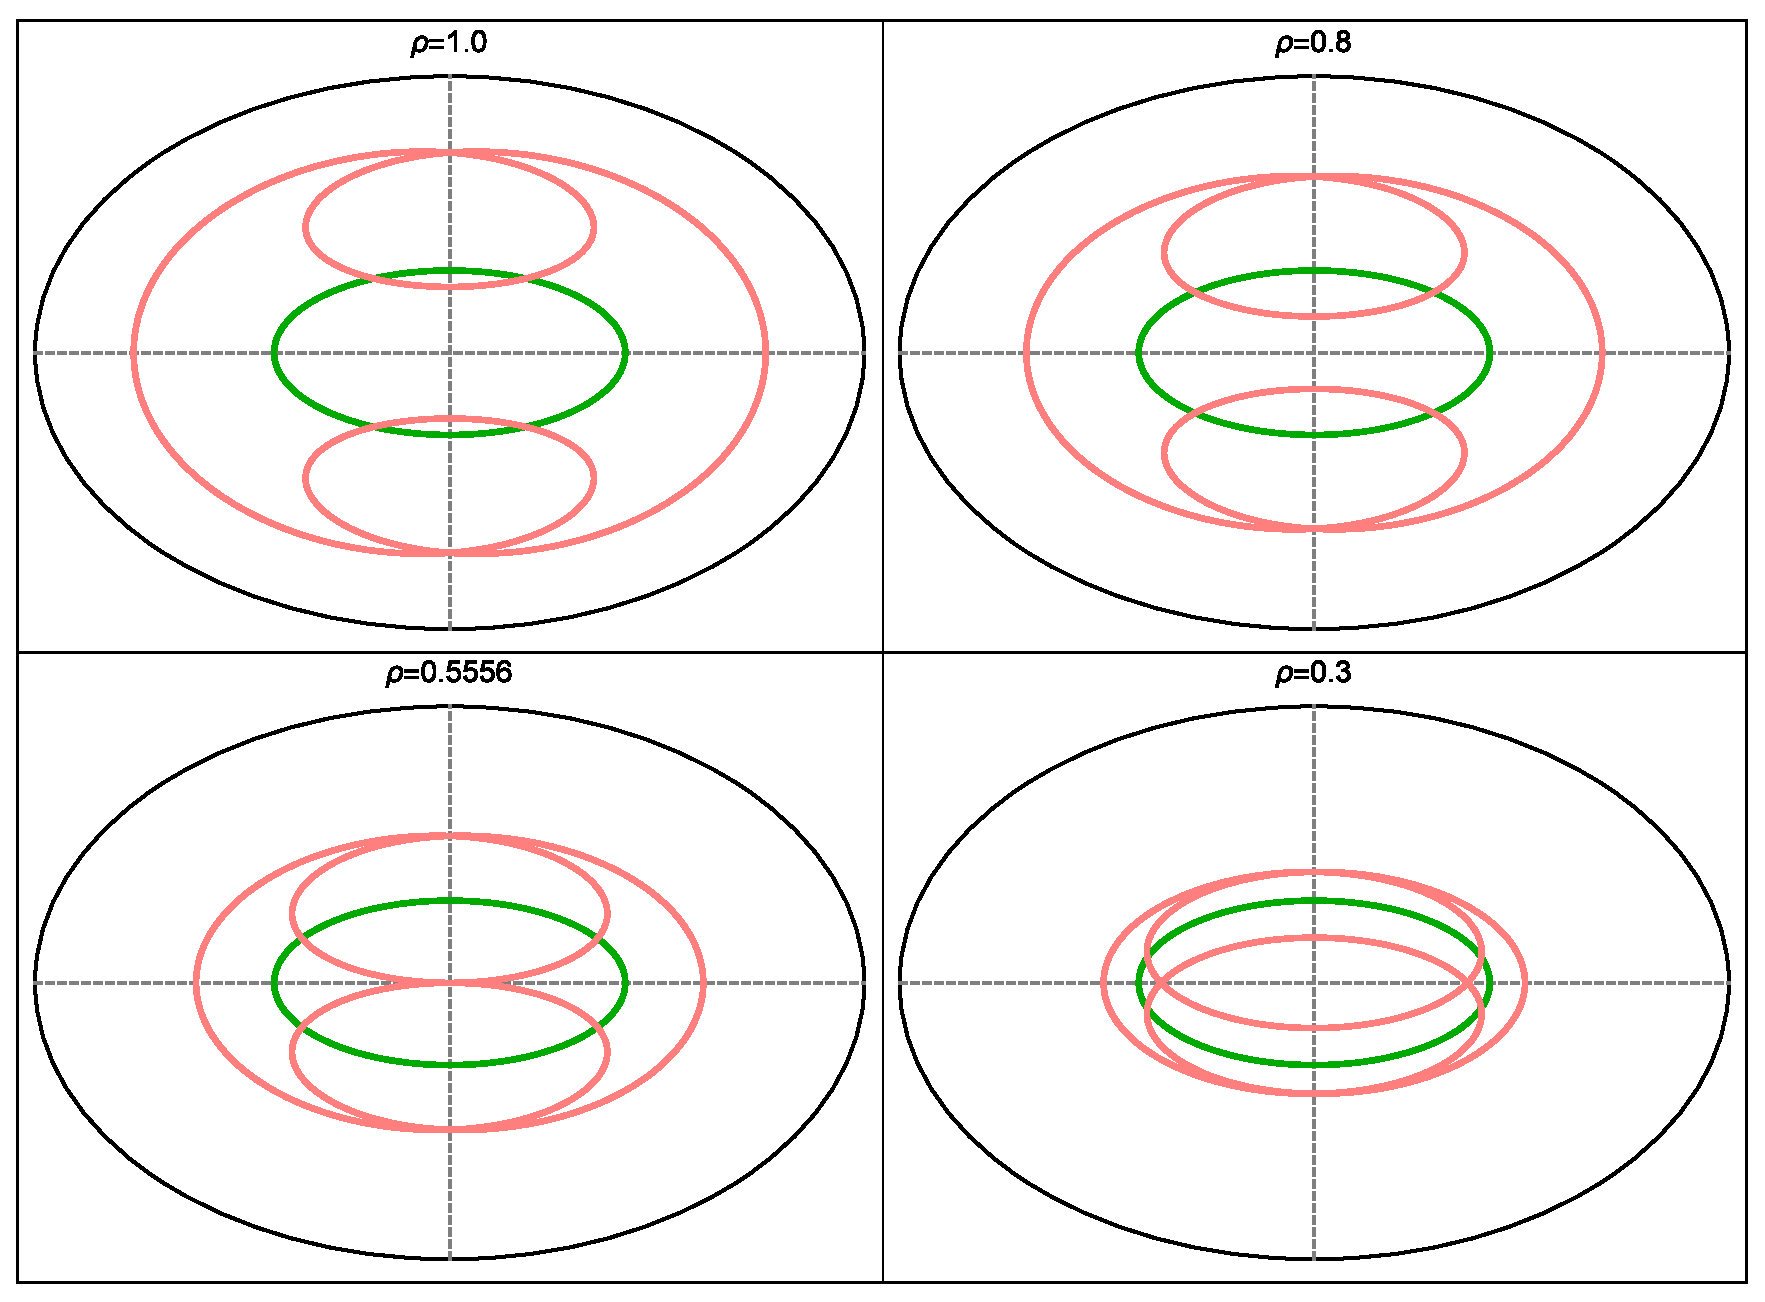
\includegraphics[width=\textwidth]{pics_05_110_conv_inc_pedal}
    \caption{The locus (pink) of convex combination $Y_1$ of the incenter and an intouchpoint at different values of $\rho$. The elliptic locus of the incenter appears in all four frames (green). When $\rho=1$ (top left), one obtains the original two-lobed locus of the intouchpoints (pink). As $\rho$ decreases (top right, bottom left), the two lobes approach each other and at some point touch. Decreasing $\rho$ further still causes loves to self-intersect and contain the ellipse pair center. As $\rho$ approaches zero (bottom right), the lobes further interpenetrate and when $\rho=0$ (not shown), they collapse to the elliptic locus of the incenter (green). \href{https://youtu.be/3Gr3Nh5-jHs}{Video 1}, \href{https://youtu.be/HZFjkWD_CnE}{Video 2}}
    \label{fig:05-inc-wind3}
\end{figure}
